% ==================================================================
%  RESULTADOS - Proyecto Final: Simulador de Filtros IIR
% ==================================================================

\subsection{Filtro Pasa Bajas ($f_c = 85$ Hz)}

Para evaluar el funcionamiento del filtro pasa bajas de primer orden, se enviaron desde MATLAB los coeficientes calculados previamente mediante la transformación bilineal ($A_0 = 0.0323$, $A_1 = 0.0323$, $B_1 = 0.9354$). La comunicación Bluetooth con el módulo HC-05 fue exitosa, como se ve en la terminal de comandos, permitiendo actualizar la frecuencia de la onda cuadrada generada en la Raspberry en tiempo real.

\begin{figure}[H]
    \centering
    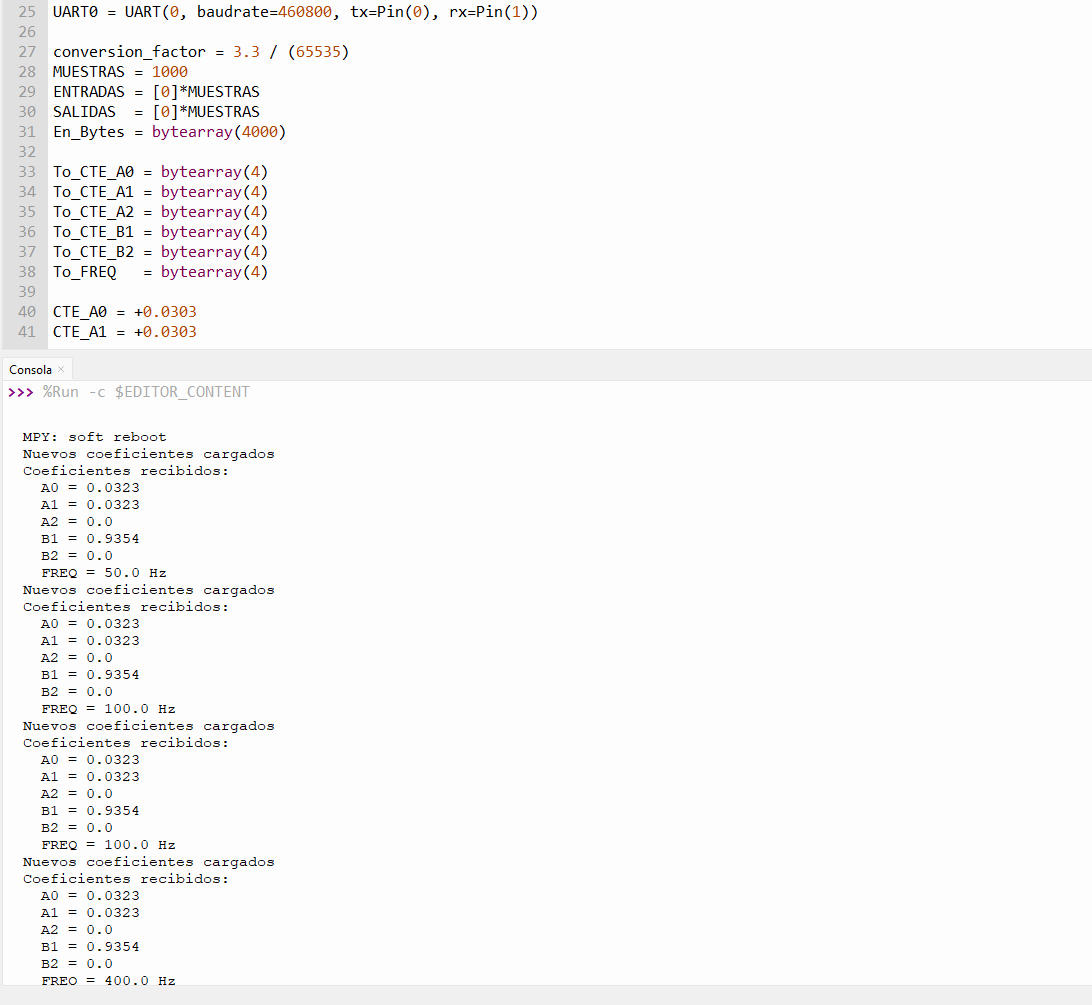
\includegraphics[width=0.93\textwidth]{img/filtropasabajas/PasaBajas_Consola.png}
    \caption{Consola de MATLAB mostrando el envío de los coeficientes del filtro pasa bajas y las distintas frecuencias de prueba.}
    \label{fig:pb_consola}
\end{figure}

A continuación, presentamos las gráficas comparativas entre la señal de entrada $U(k)$ (onda cuadrada azul) y la señal de salida $Y(k)$ (señal filtrada roja) para los diferentes casos de prueba capturados a 50 Hz, 100 Hz y 200 Hz.

\subsubsection{Prueba con $f = 50$ Hz ($f < f_c$)}

Al aplicar una frecuencia menor a la frecuencia de corte teórica ($85\text{ Hz}$), la señal se encuentra dentro de la banda de paso. En la siguiente observamos que el filtro atenúa los armónicos de alta frecuencia de los flancos de la onda cuadrada, dando como resultado una salida con la clásica curva exponencial de carga y descarga, pero logrando alcanzar casi la amplitud máxima de la señal de entrada.

\begin{figure}[H]
    \centering
    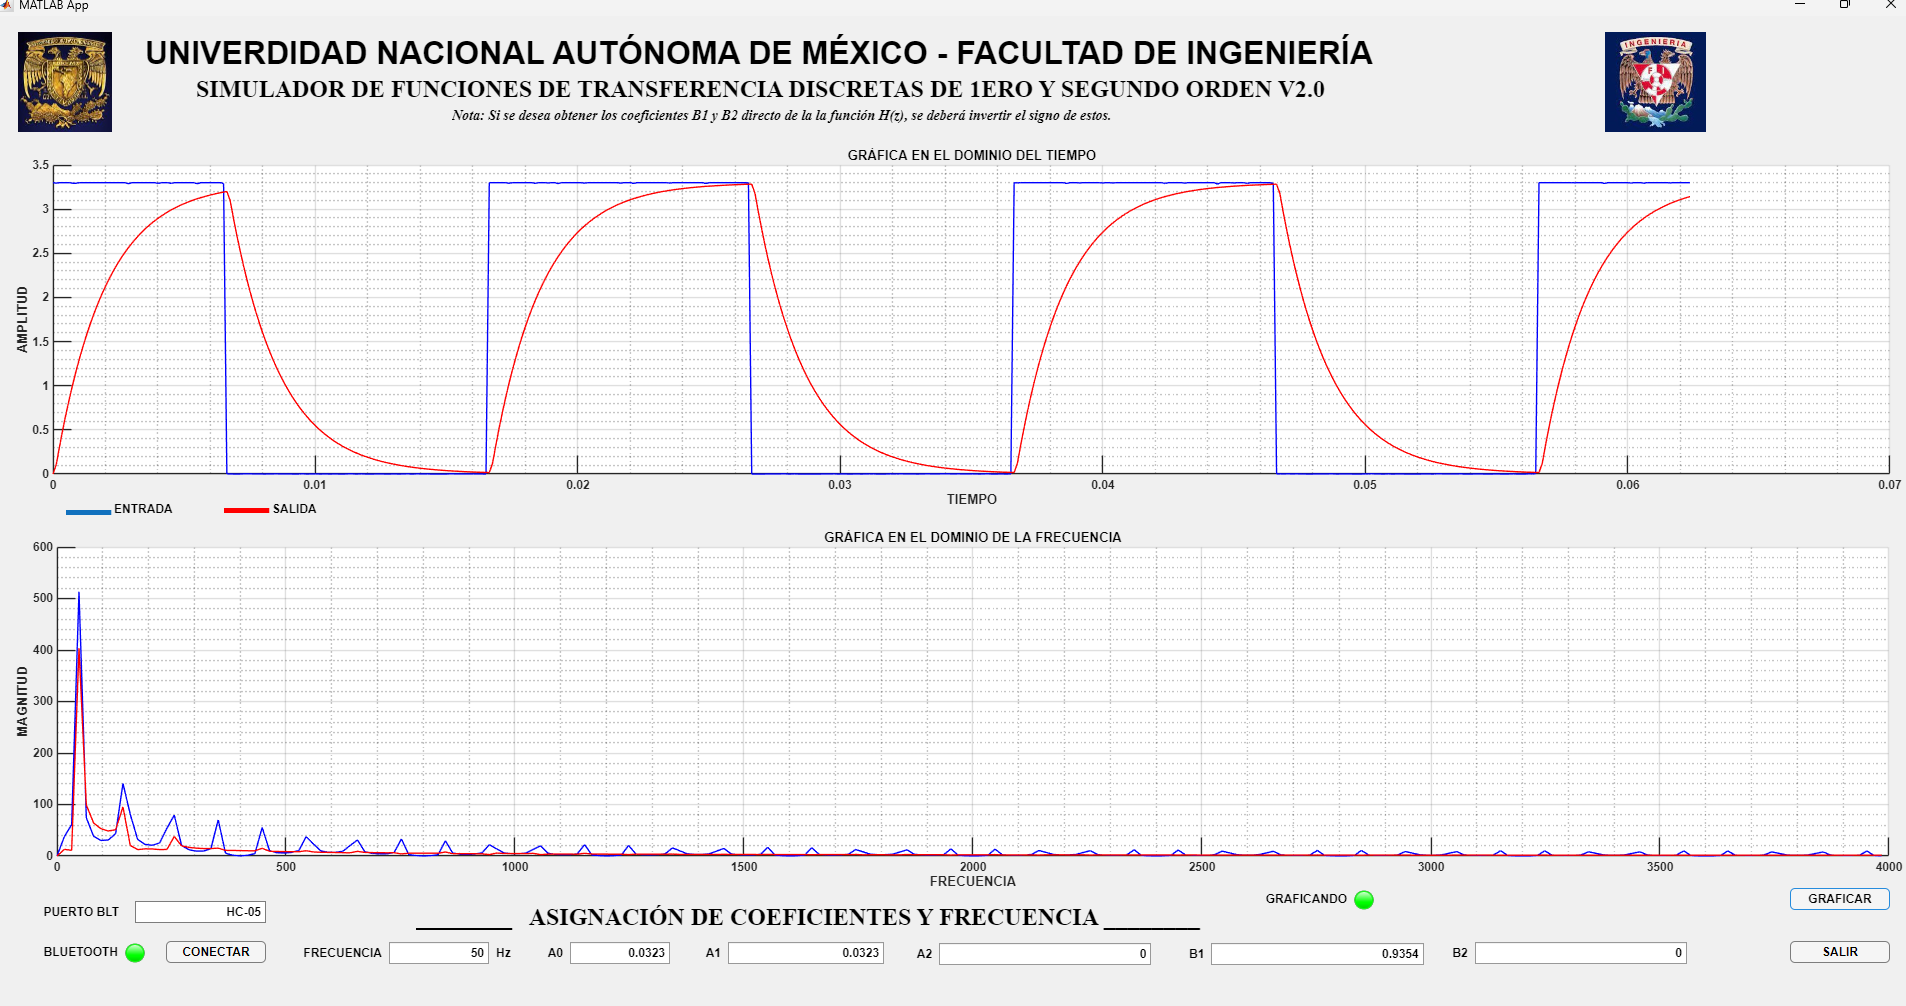
\includegraphics[width=1\textwidth]{img/filtropasabajas/PasaBajas_Res1.png}
    \caption{Respuesta del filtro pasa bajas a una entrada de 50 Hz. Se observa el seguimiento de la señal con distorsión exponencial típica de un sistema de primer orden.}
    \label{fig:pb_50hz}
\end{figure}

\subsubsection{Prueba con $f = 100$ Hz ($f > f_c$)}

La segunda prueba la hicimos dando una señal de $100\text{ Hz}$. Al haber superado la frecuencia de corte de $85\text{ Hz}$, la señal entra en la banda de rechazo del filtro. Y la siguiente imagen demuestra que la señal filtrada roja sufre una atenuación visible y ya no logra alcanzar el nivel de voltaje de la señal de entrada, debido a que el sistema no tiene tiempo suficiente para cargar antes del siguiente cambio de estado.

\begin{figure}[H]
    \centering
    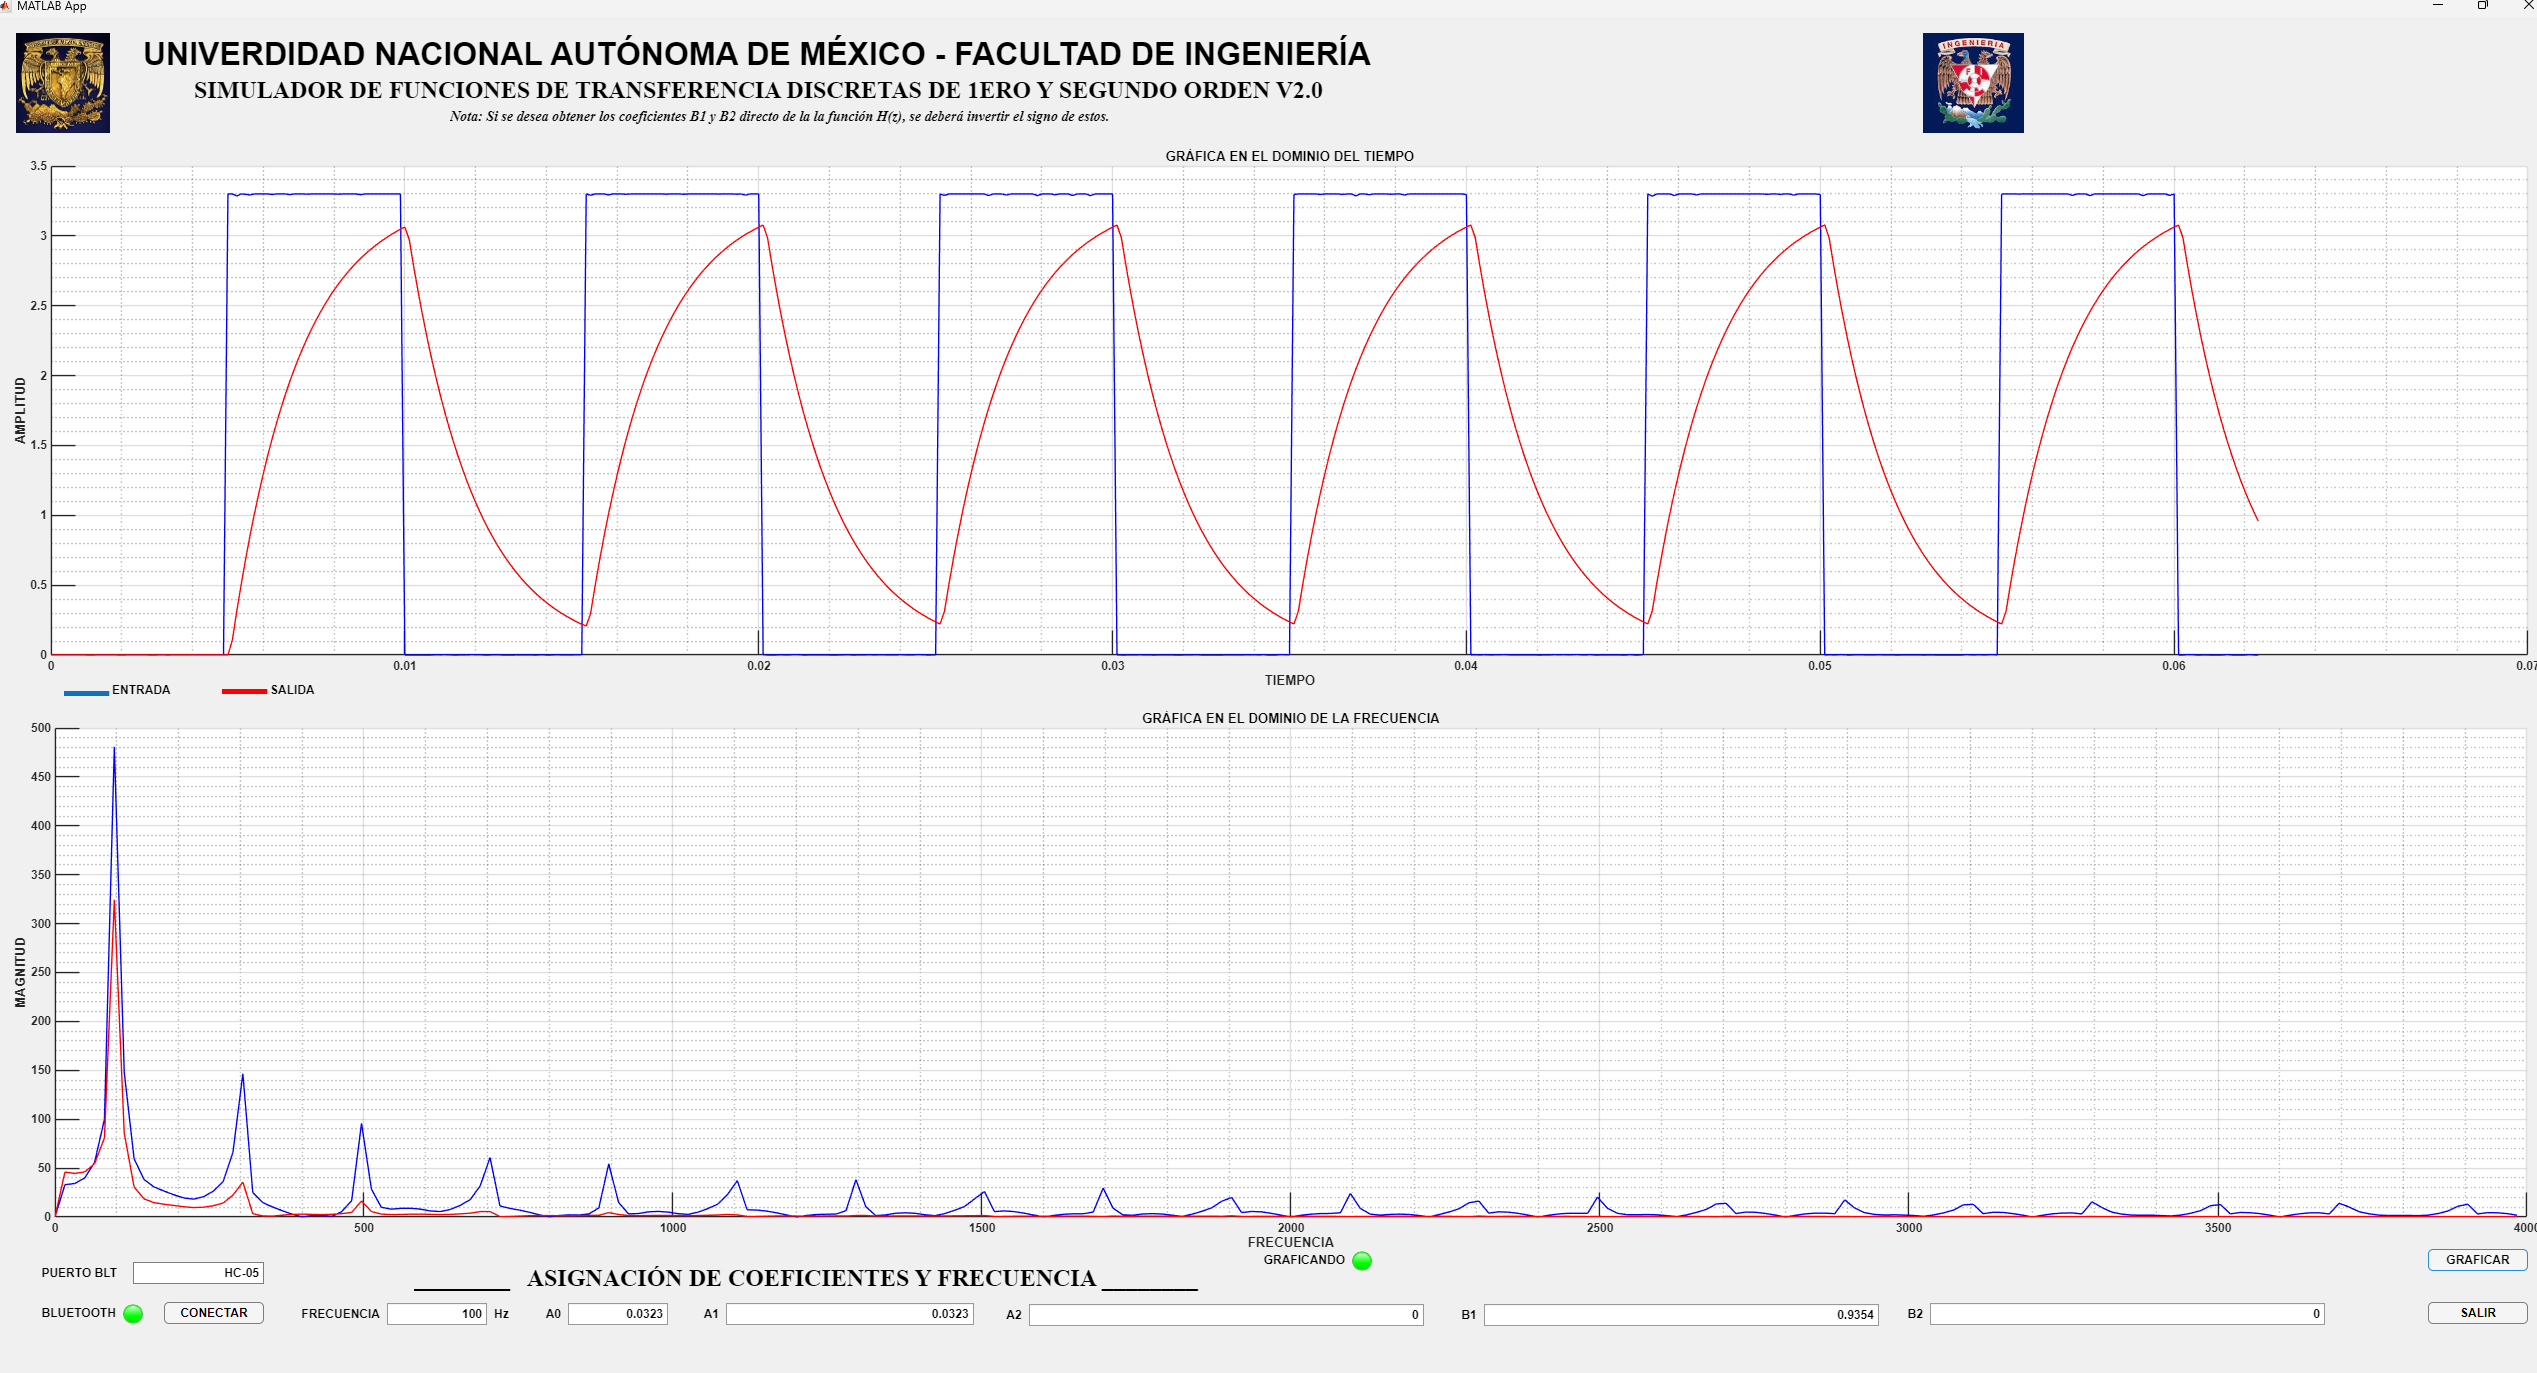
\includegraphics[width=1\textwidth]{img/filtropasabajas/PasaBajas_Res2.png}
    \caption{Respuesta del filtro pasa bajas a una entrada de 100 Hz. Se aprecia una atenuación notable al haber superado la frecuencia de corte.}
    \label{fig:pb_100hz}
\end{figure}

\subsubsection{Prueba con $f = 200$ Hz ($f \gg f_c$)}

Ahora, se aumentó la frecuencia de la señal de entrada a $200\text{ Hz}$. Estando considerablemente por encima de la frecuencia de corte, el comportamiento esperado era una atenuación más significativa. En la imagen podemos ver este rechazo, en la salida $Y(k)$ se presenta una amplitud sumamente reducida y se asemeja más como a una onda triangular pequeña, y es aqui donde podemos ver la capacidad del filtro para suprimir componentes de alta frecuencia.

\begin{figure}[H]
    \centering
    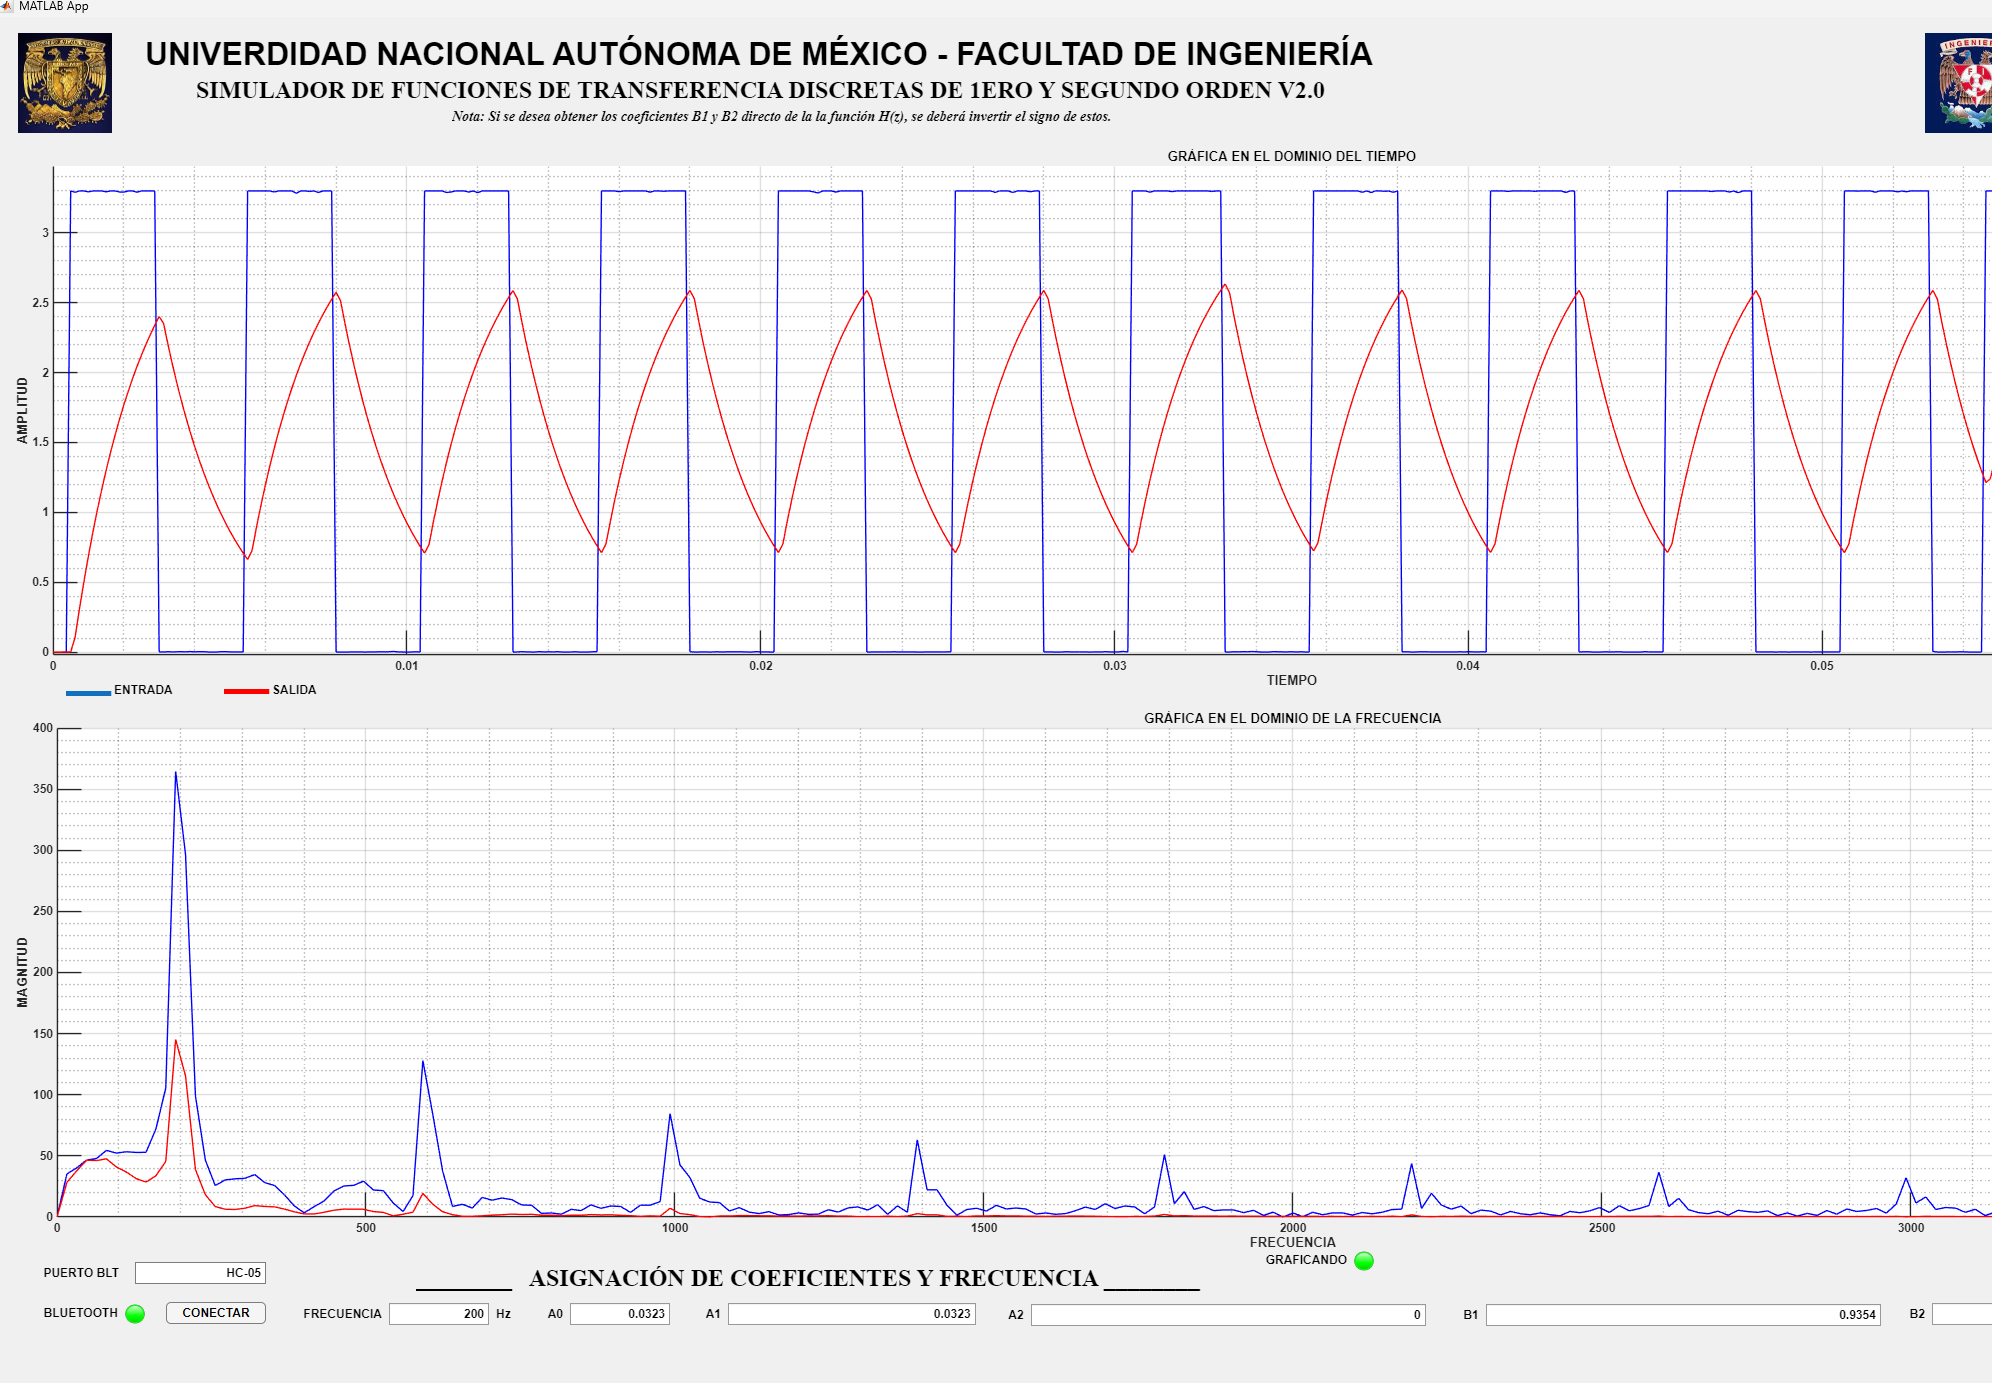
\includegraphics[width=1\textwidth]{img/filtropasabajas/PasaBajas_Res3.png}
    \caption{Respuesta del filtro pasa bajas a una entrada de 200 Hz. Muestra una atenuación severa, filtrando casi en su totalidad la señal.}
    \label{fig:pb_200hz}
\end{figure}


\subsection{Filtro Pasa Altas ($f_c = 480$ Hz)}

De manera similar al caso anterior, se enviaron desde MATLAB los coeficientes correspondientes al filtro pasa altas de primer orden ($A_0 = 0.8397$, $A_1 = -0.8397$, $B_1 = 0.6794$). En la consola podemos ver la correcta recepción de estos valores y la actualización de las frecuencias a probar.

\begin{figure}[H]
    \centering
    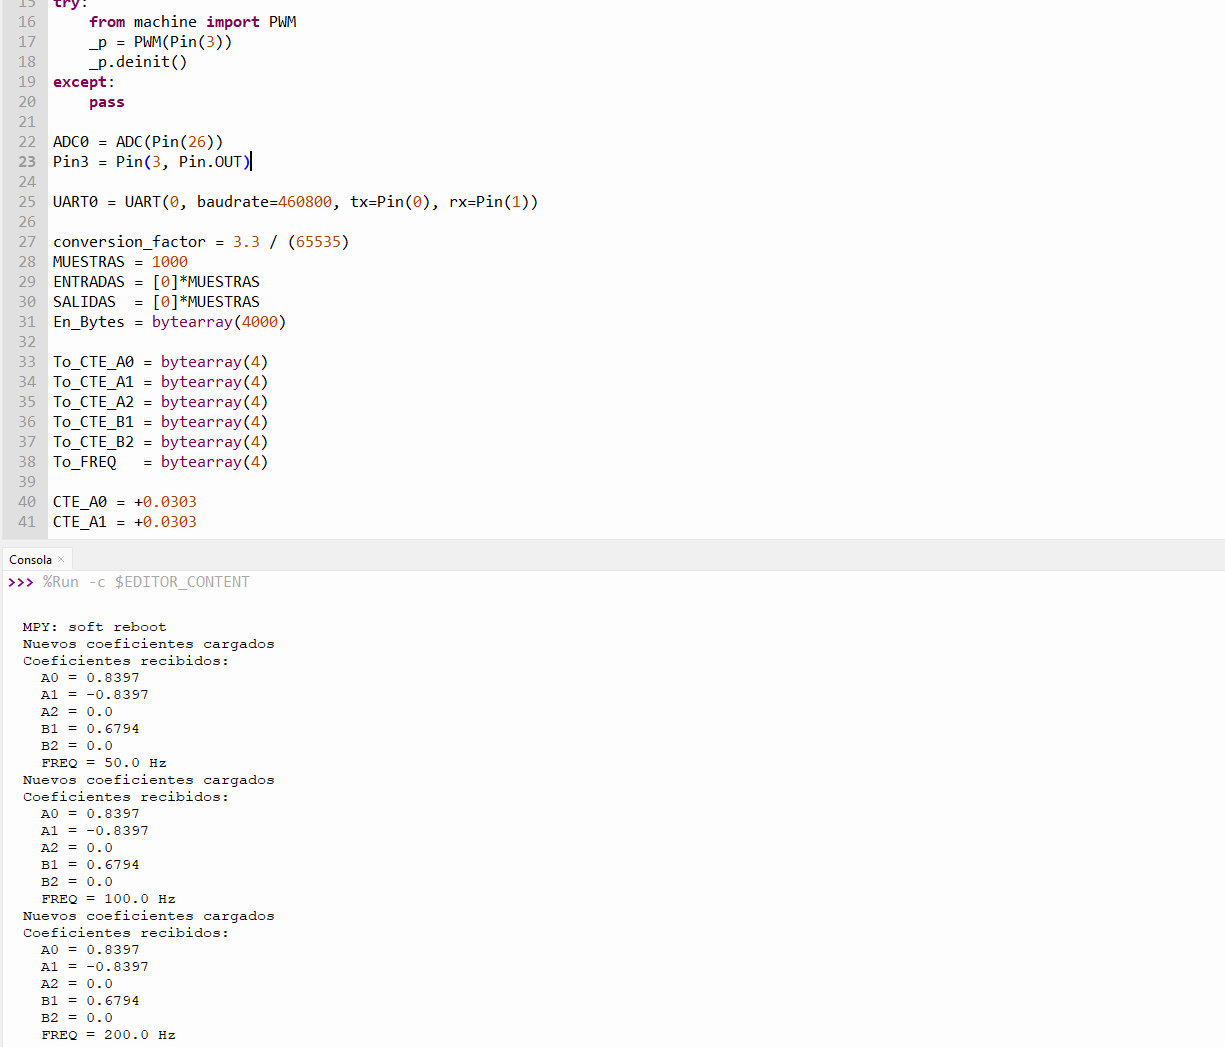
\includegraphics[width=1\textwidth]{img/filtropasaaltas/PasaAltas_Consola.png}
    \caption{Consola de MATLAB mostrando la carga exitosa de los coeficientes del filtro pasa altas y las frecuencias enviadas.}
    \label{fig:pa_consola}
\end{figure}

Para este filtro, la frecuencia de corte teórica es de $480\text{ Hz}$. Dado que las frecuencias de prueba (50 Hz, 100 Hz y 200 Hz) están por debajo de este valor, la componente fundamental de la señal cuadrada se encuentra en la banda de atenuación en los tres casos. Sin embargo, debido a que los flancos abruptos de la onda cuadrada están compuestos por armónicos de muy alta frecuencia, el filtro permitirá el paso de estos transitorios, comportándose como un circuito derivador.

\subsubsection{Prueba con $f = 50$ Hz ($f \ll f_c$)}

Al aplicar una frecuencia de $50\text{ Hz}$, estando muy por debajo de la frecuencia de corte, la atenuación de la señal original es muy fuerte. En la imagen se observa claramente que el filtro elimina por completo las partes planas (constantes o de baja frecuencia) de la onda cuadrada. Solo sobreviven los cambios bruscos de estado, generando picos de voltaje que decaen rápidamente a cero entre un flanco y otro.

\begin{figure}[H]
    \centering
    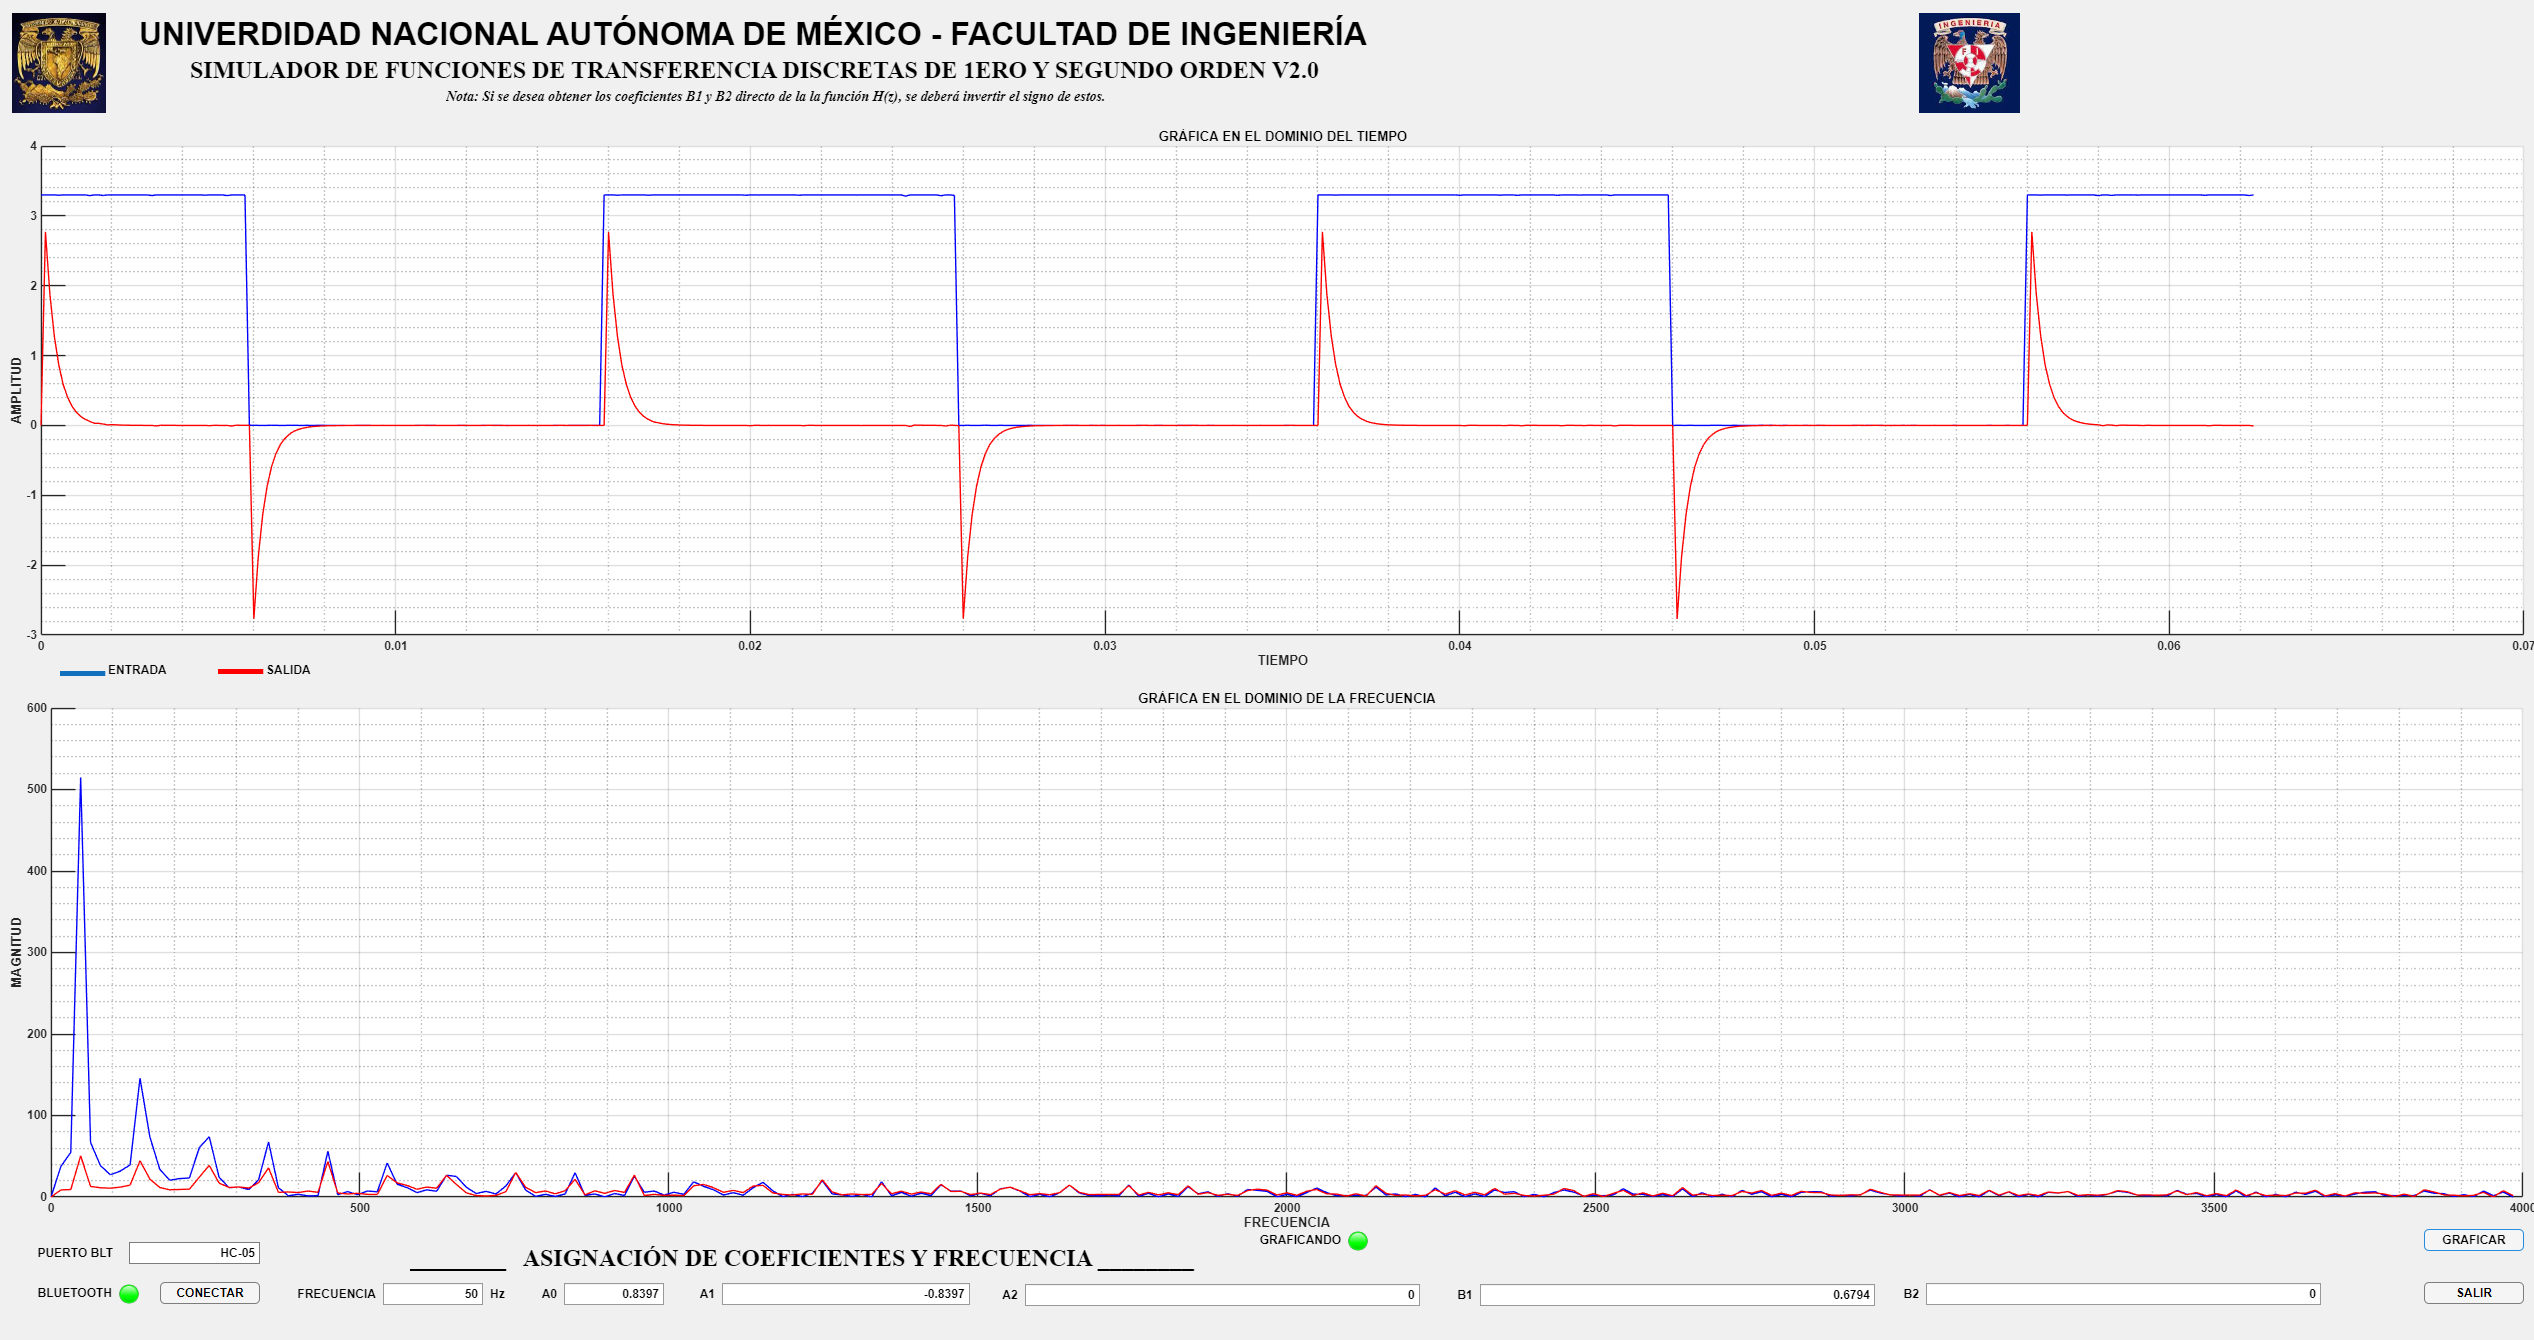
\includegraphics[width=1\textwidth]{img/filtropasaaltas/PasaAltas_Res1.png}
    \caption{Respuesta del filtro pasa altas a 50 Hz. Se observa una atenuación fuerte de la componente fundamental, dejando pasar únicamente los transitorios de los flancos.}
    \label{fig:pa_50hz}
\end{figure}

\subsubsection{Prueba con $f = 100$ Hz ($f < f_c$)}

Al incrementar la frecuencia a $100\text{ Hz}$, seguimos dentro de la banda de atenuación. El comportamiento es el mismo: la señal filtrada roja muestra exclusivamente las respuestas transitorias en cada cambio de flanco de la señal azul de entrada. Al ser el periodo más corto que en la prueba anterior, los picos se presentan con mayor frecuencia en la gráfica, pero la amplitud de las partes planas sigue siendo rechazada y llevada a cero.

\begin{figure}[H]
    \centering
    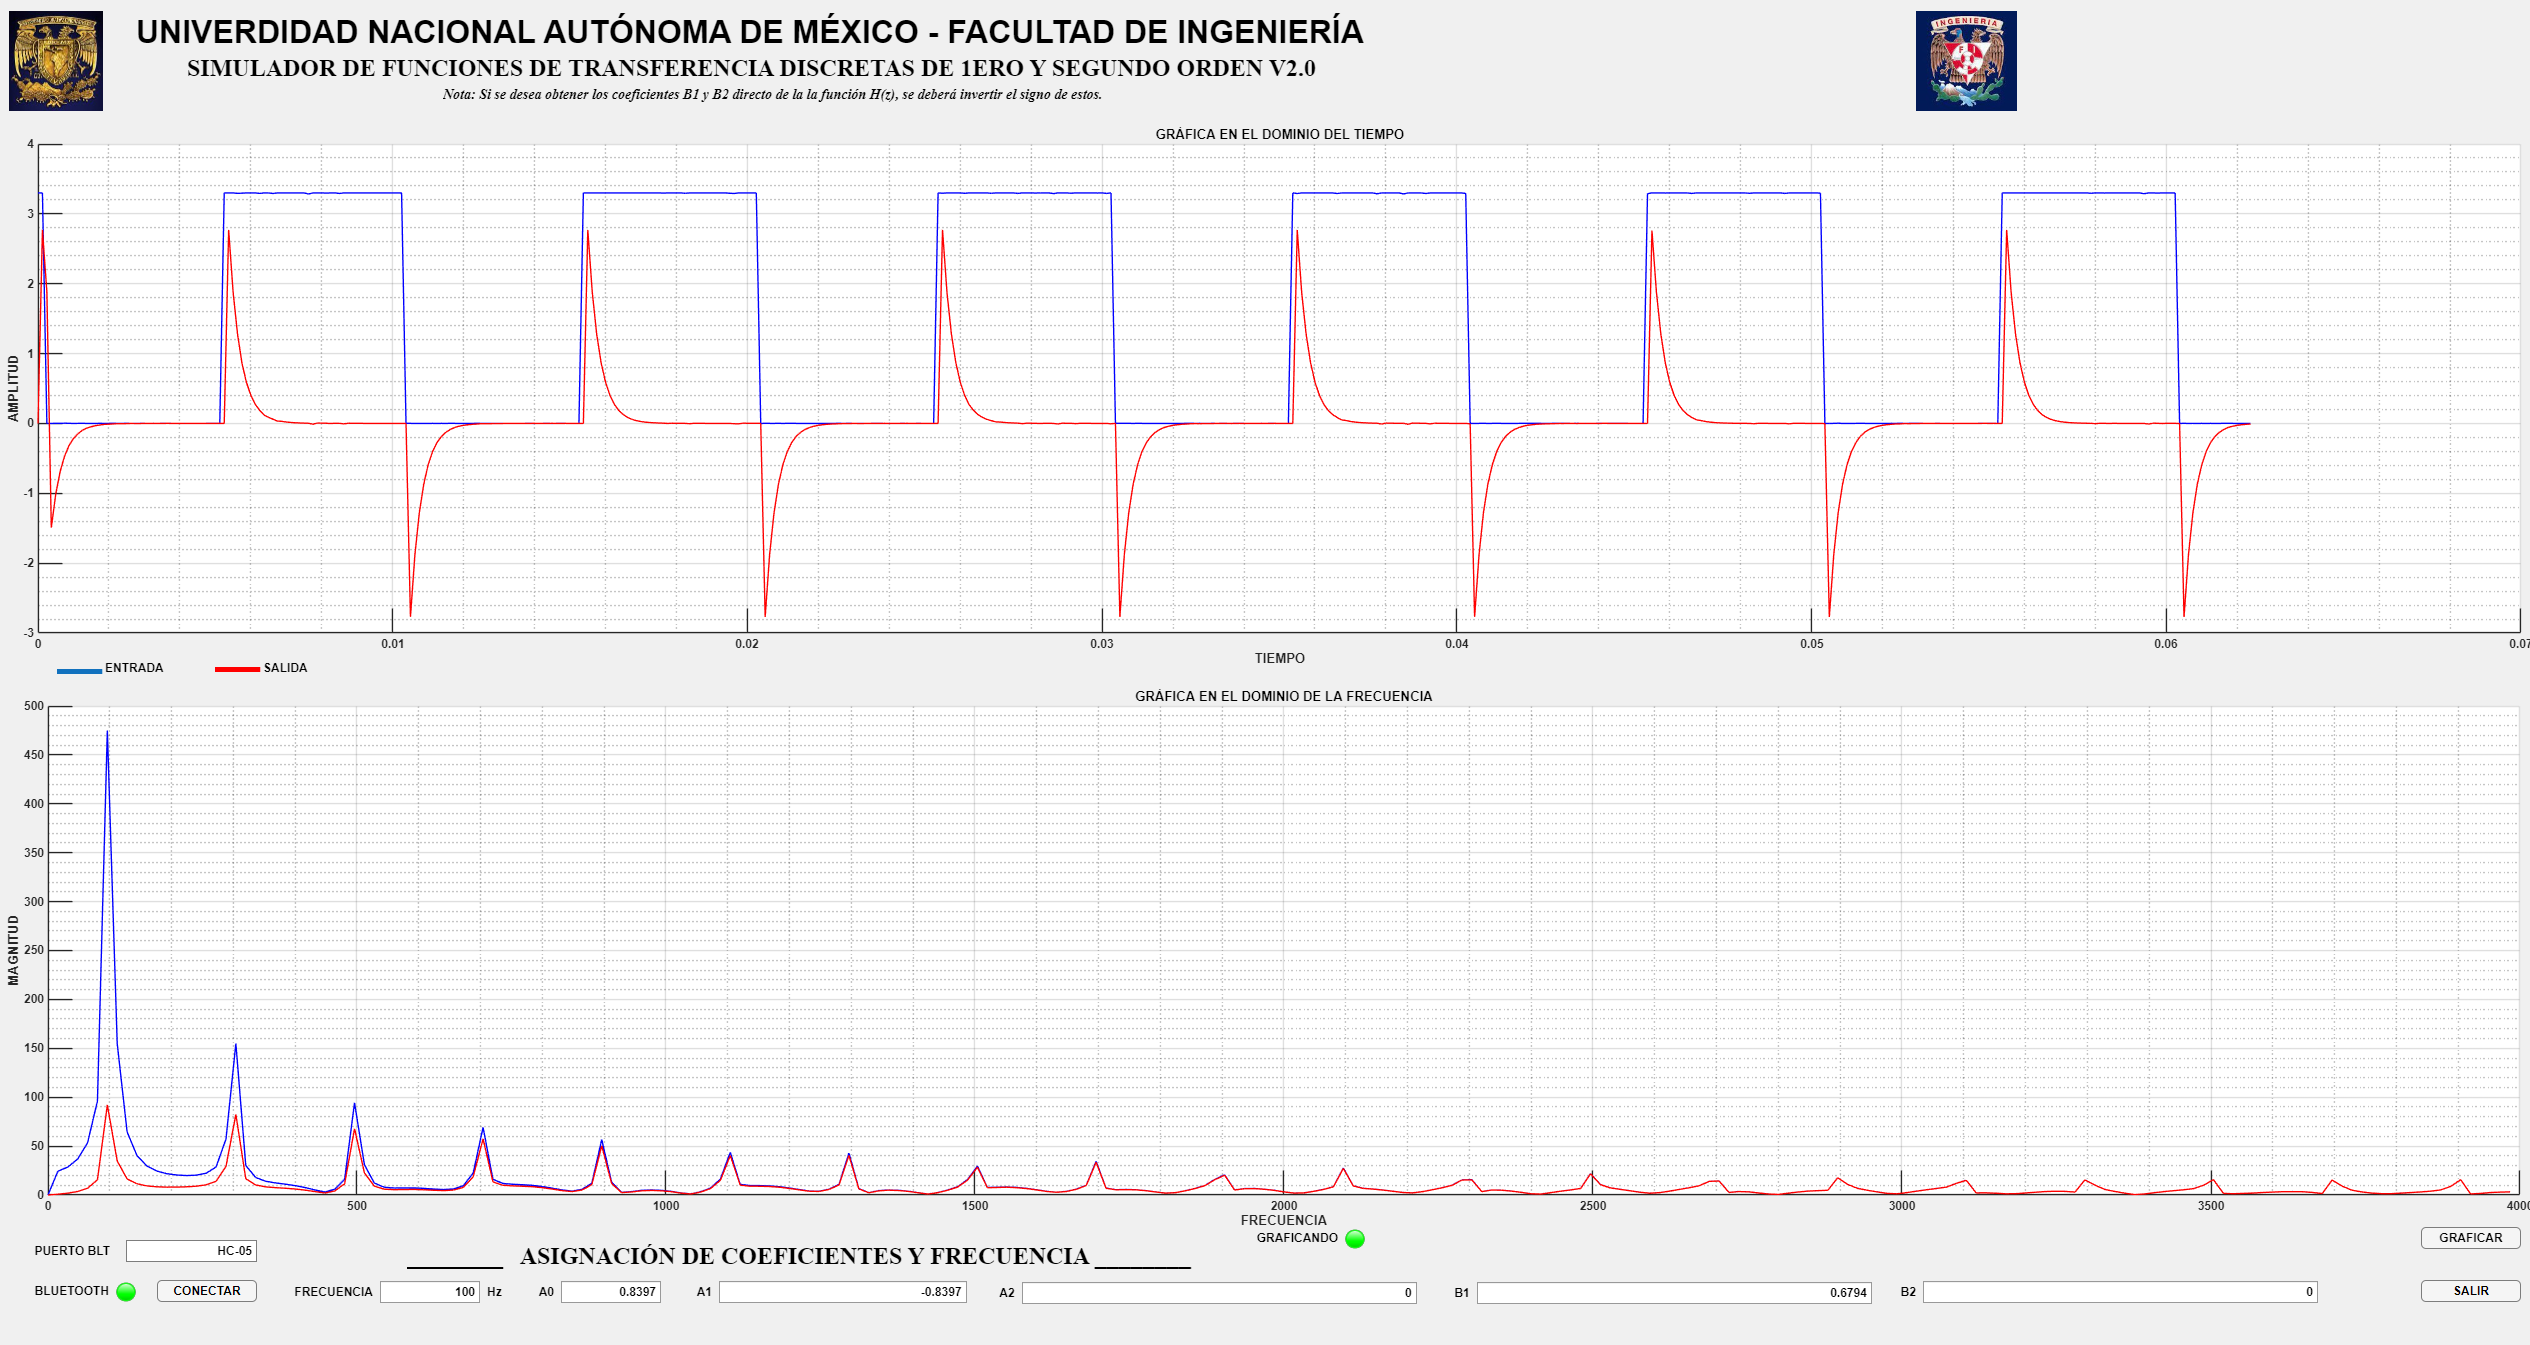
\includegraphics[width=1\textwidth]{img/filtropasaaltas/PasaAltas_Res2.png}
    \caption{Respuesta del filtro pasa altas a 100 Hz. Las partes planas de la onda cuadrada continúan siendo filtradas exitosamente.}
    \label{fig:pa_100hz}
\end{figure}

\subsubsection{Prueba con $f = 200$ Hz ($f < f_c$)}

En la última prueba a $200\text{ Hz}$, aunque nos acercamos un poco más a la frecuencia de corte, todavía nos encontramos por debajo de los $480\text{ Hz}$. La gráfica reafirma la estabilidad del filtro: actúa de manera consistente eliminando las componentes de baja frecuencia y permitiendo el paso de los armónicos superiores que conforman las transiciones de la onda cuadrada de entrada.

\begin{figure}[H]
    \centering
    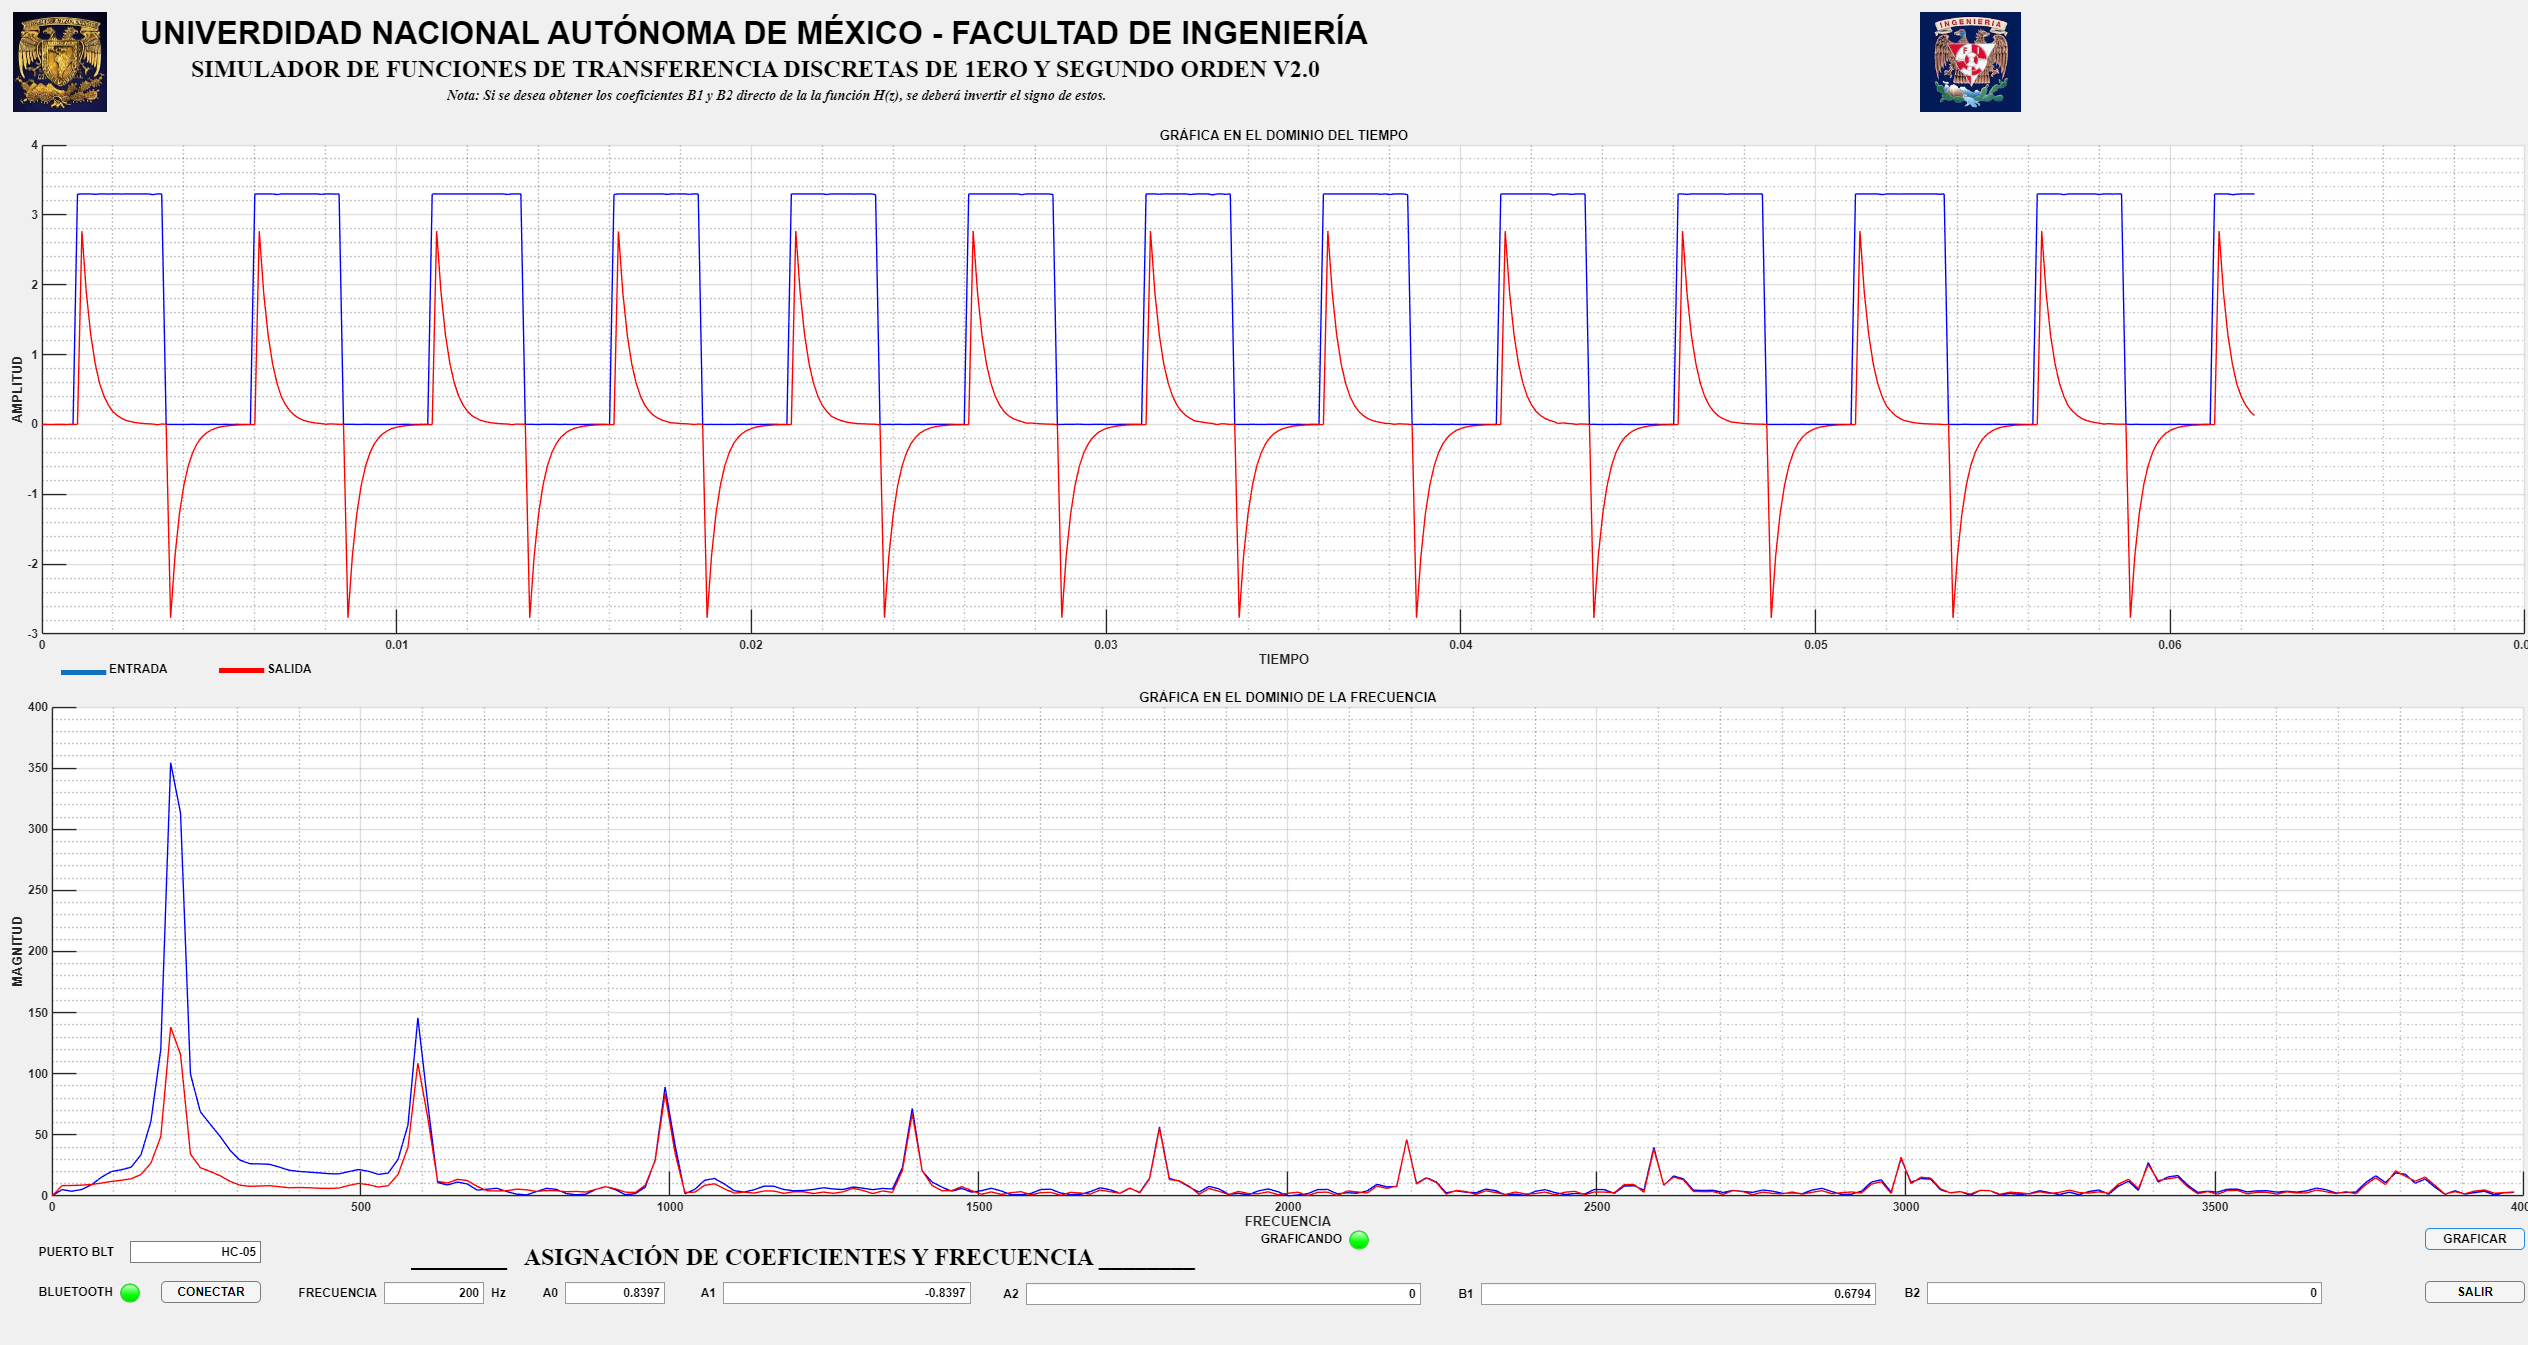
\includegraphics[width=1\textwidth]{img/filtropasaaltas/PasaAltas_Res3.png}
    \caption{Respuesta del filtro pasa altas a 200 Hz. El comportamiento derivador se mantiene estable, destacando los cambios rápidos de la señal.}
    \label{fig:pa_200hz}
\end{figure}




\subsection{Filtro Pasa Banda ($f_o = 580$ Hz, $BW = 45$ Hz)}

Para la implementación del filtro pasa banda, se enviaron al sistema los coeficientes calculados para obtener una frecuencia central de $580\text{ Hz}$ con un ancho de banda de $45\text{ Hz}$, estos coeficientes fueron $A_0 = 0.01832$, $A_1 = 0.0$, $A_2 = -0.01832 $, $B_1 = 1.76283 $ $B_2 = -0.96337$ y de igual forma que en los casos anteriores la comunicación con el módulo HC-05 fue satisfactoria, permitiendo la carga de los parámetros y la sintonización del filtro en tiempo real, según se verifica en la imagen de abajo donde se muestra la consola.

\begin{figure}[H]
    \centering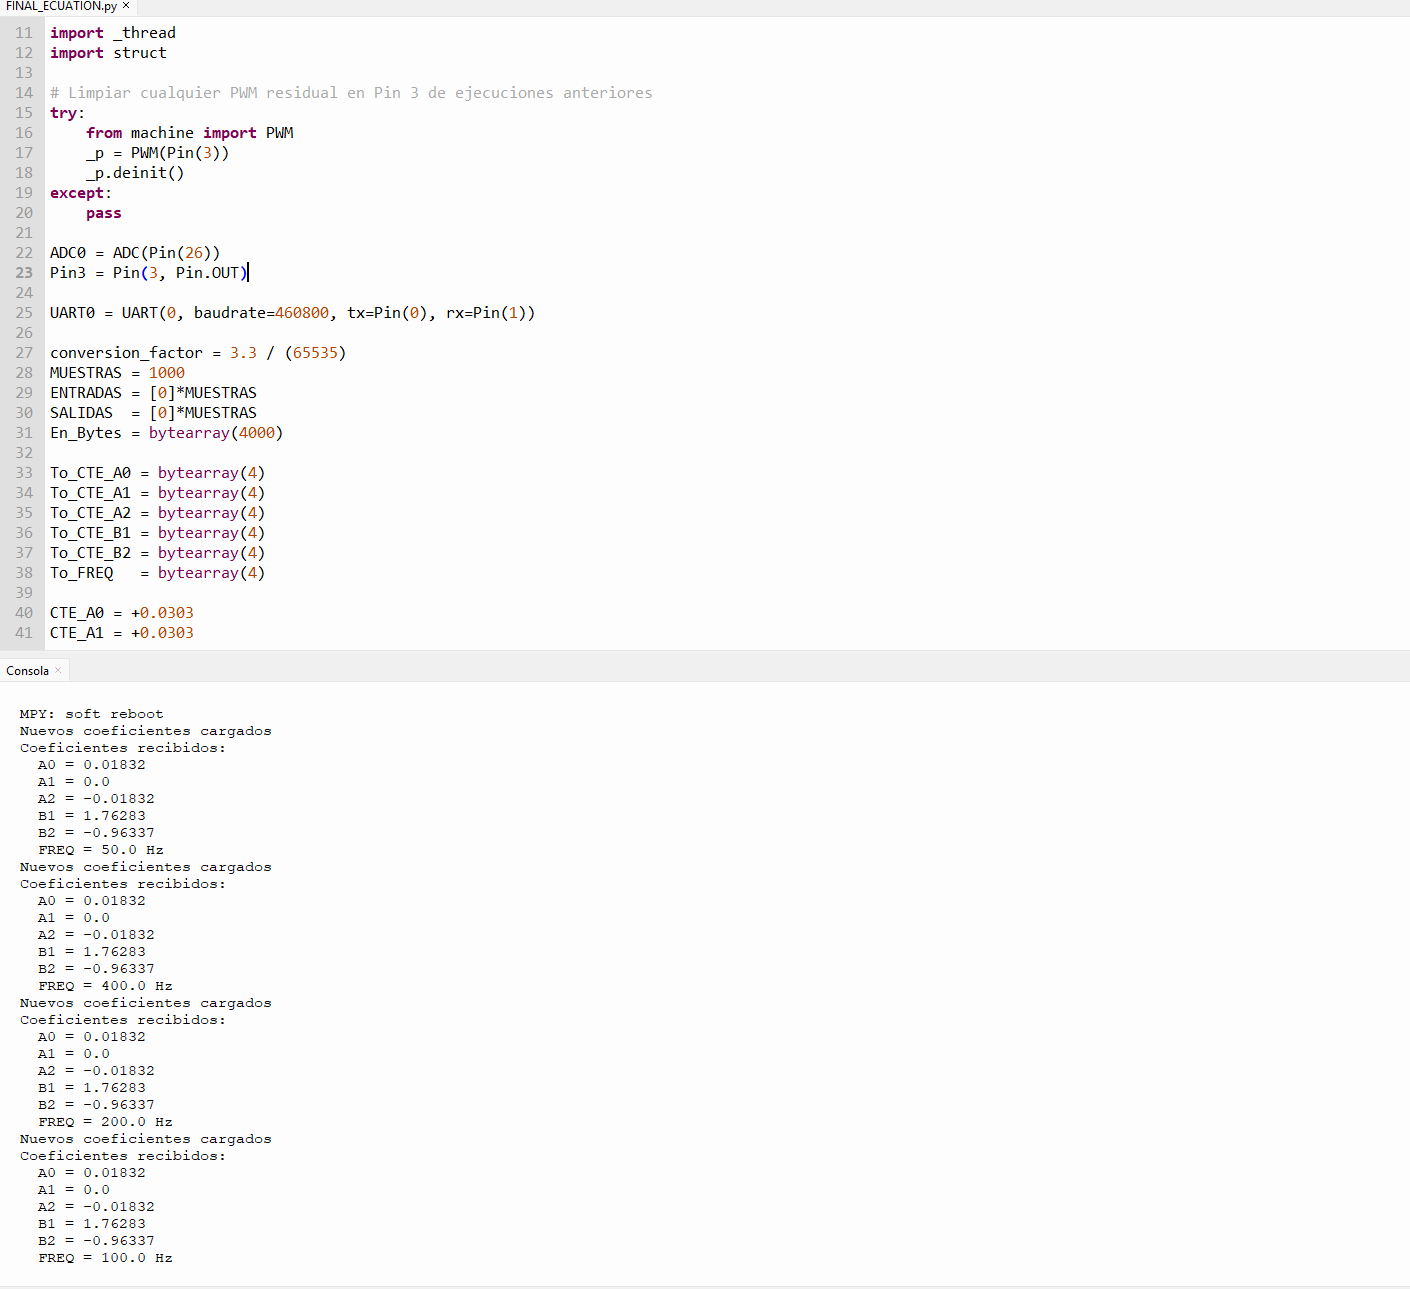
\includegraphics[width=1\textwidth]{img/filtropasobandas/PasaBanda_Consola.png}
    \caption{Consola de MATLAB mostrando la carga de los coeficientes para el filtro pasa banda y la recepción de las distintas frecuencias de prueba.}\label{fig:pbanda_consola}\end{figure}
    
Dado que la frecuencia central de diseño de $580\text{ Hz}$ está fuera del rango de las frecuencias de prueba utilizadas anteriormente, por lo tanto el filtro se comporta de manera selectiva frente a la entrada. A continuación, analizamos el comportamiento del filtro ante diferentes señales.

\subsubsection{Prueba con $f = 50$ Hz ($f < f_o$)}

Al aplicar una frecuencia de $50\text{ Hz}$, la cual se encuentra significativamente por debajo de la frecuencia de corte inferior de la banda de paso, observamos que el filtro atenúa drásticamente la señal. Como se aprecia en la figura, la salida $Y(k)$ presenta una amplitud mínima, confirmando que las componentes de baja frecuencia son bloqueadas eficazmente por la sección pasa altas del filtro, dejando pasar únicamente una mínima fracción de la señal original.

\begin{figure}[H]
    \centering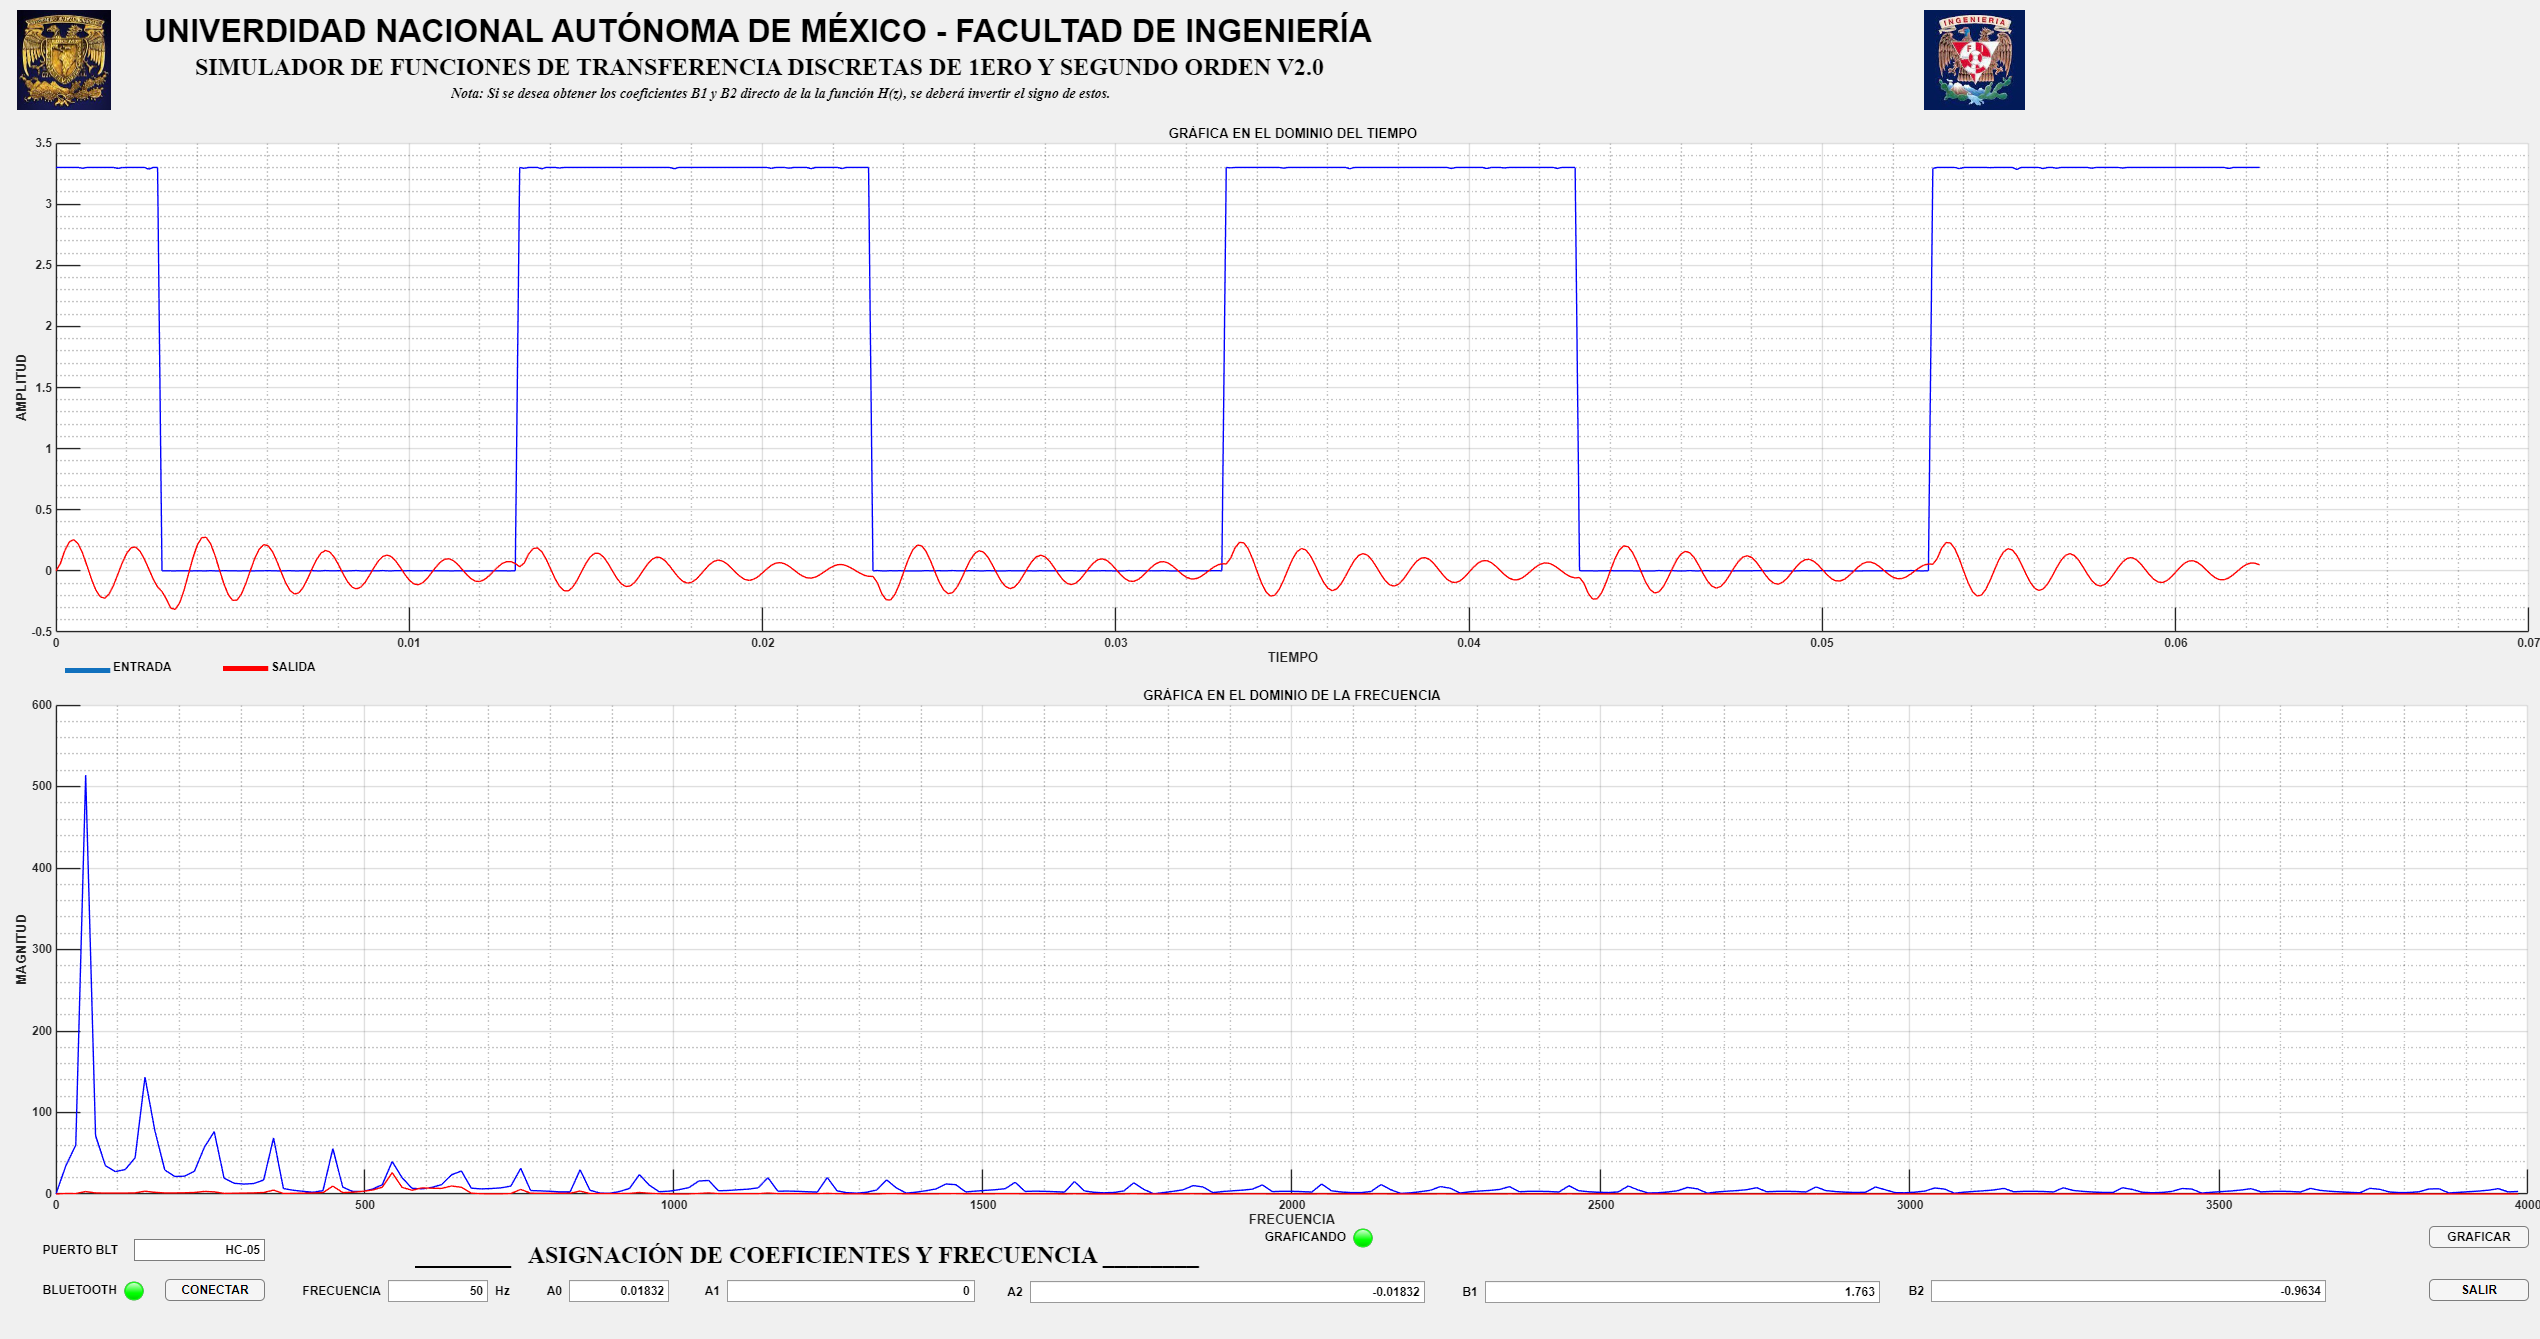
\includegraphics[width=1\textwidth]{img/filtropasobandas/PasaBanda_Res1.png}
    \caption{Respuesta del filtro pasa banda a 50 Hz. Se observa una fuerte atenuación, ya que la frecuencia de entrada está muy alejada de la banda de paso.}\label{fig:pbanda_50hz}
\end{figure}
    
\subsubsection{Prueba con $f = 100$ Hz ($f \approx f_o$)}

Al incrementar la frecuencia a $100\text{ Hz}$, aunque todavía nos encontramos lejos de la frecuencia central de diseño, el filtro comienza a mostrar una respuesta ligeramente menos atenuada que en la prueba anterior. A pesar de estar en la zona de transición, la salida $Y(k)$ nos muestra la selectividad del sistema, permitiendo el paso de una mayor amplitud de la señal de entrada a medida que nos acercamos a la banda de paso.

\begin{figure}[H]
    \centering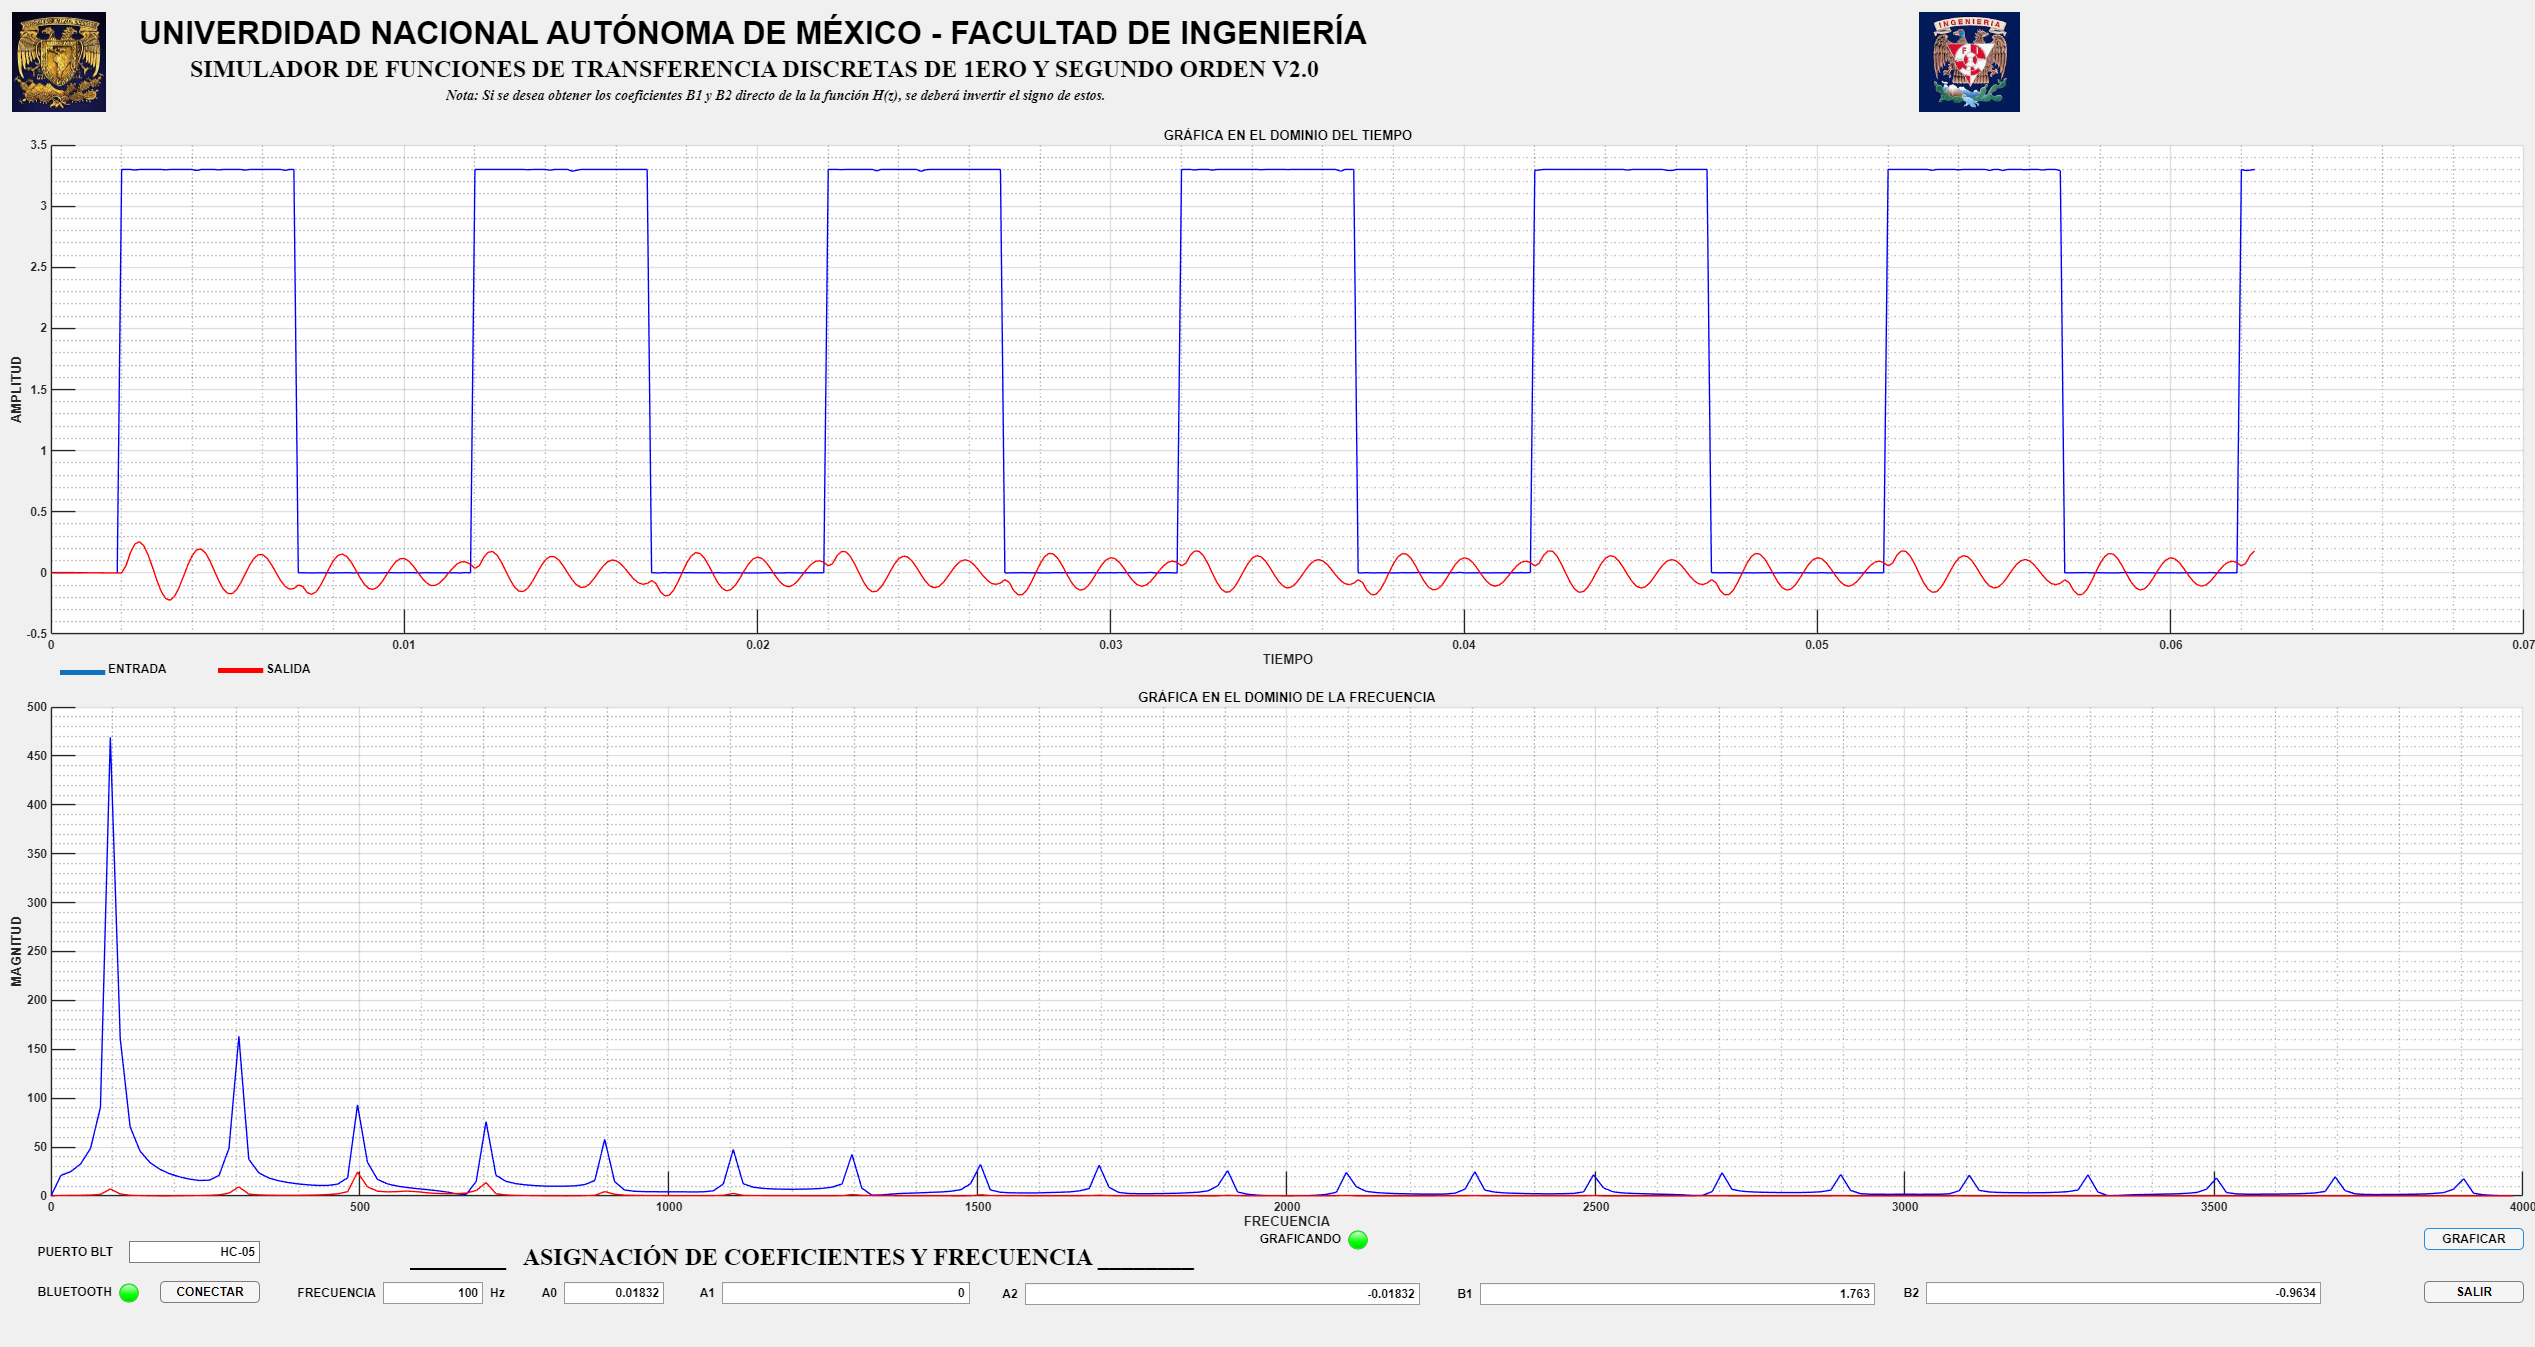
\includegraphics[width=1\textwidth]{img/filtropasobandas/PasaBanda_Res2.png}
    \caption{Respuesta del filtro pasa banda a 100 Hz. Se observa una atenuación menor en comparación a la prueba de 50 Hz al acercarse progresivamente a la frecuencia central.}\label{fig:pbanda_100hz}
\end{figure}
